We will now present a possible usage scenario of some algorithms in the data matching library.
We have gathered two weather dataframes (one recording data in Delhi, India and the other in Seattle, US) from independent
sources on Kaggle~~\cite{kaggleDailyDelhiClimate,kaggleSeattleWeather} and are now interested in learning more about them
as well as verifying some basic properties before we insert them in some analysis and visualization software.
First of all, we will generate the metadata.
Fig~\ref{fig:daily_delhi_climate} displays the metadata of the Delhi weather report and fig~\ref{fig:seattle_weather} contains
the metadata of the Seattle report.

\begin{figure}[H]
    \centering
    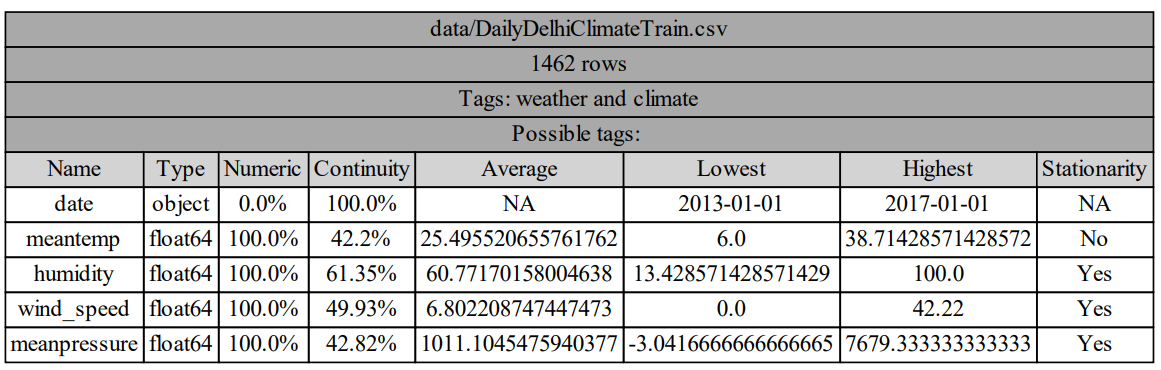
\includegraphics[width=12cm]{figures/matching_weather_data/daily_delhi_climate}
    \caption{Metadata for the ``Daily Delhi Climate'' dataframe}
    \label{fig:daily_delhi_climate}
\end{figure}

\begin{figure}[H]
    \centering
    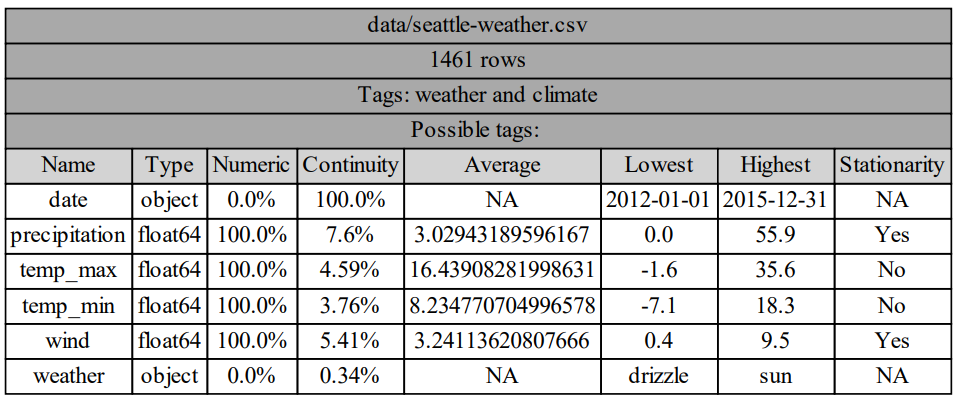
\includegraphics[width=12cm]{figures/matching_weather_data/seattle_weather}
    \caption{Metadata for the ``Seattle Weather'' dataframe}
    \label{fig:seattle_weather}
\end{figure}

Looking at the minimum and maximum values of the date column, we note that observations have been recorded from January 1st
to January 1st across a number of years.

Now we will ask some questions that will help us learn more about this data.
For example, we would like to know if the unknown mean of the column \texit{meantemp} in the Delhi dataframe is equal to the
unknown mean of the column \texit{temp\_max} in the Seattle.
Intuitively, we answer ``no'' because these two cities are in vastly different regions of the world.
We will use the Two-Sample t-Test to verify our theory.
In this case, the algorithm produces a p-value much smaller than 5\% (approximately 6.82e-142), confirming that the means
are indeed not equal.

Next, we would like to know how similar the trends followed by the same two columns are.
Taking into consideration the observation from earlier, that the recordings start and end on January 1st in both dataframes
and that both cities are in the northern hemisphere, we intuitively conclude that the trends will look similar.
To verify our claim, we run the Dynamic Time Warping algorithm and obtain the distance value 112 and the resulting similarity
of 80.21\%.
This already looks like a good result, but we are not satisfied.
What does the value 112 for distance mean?
And is a similarity score of 80.21\% enough to conclude that the data can be trusted and the trends are indeed similar?
We can further solidify our beliefs by running sanity checks.
Recall that the Dynamic Time Warping algorithm uses the maximum value in the first column multiplied by the column's length
to normalize the distance to a percentage.
So, in one possible sanity test, we keep the first column as \texit{meantemp}, but run the algorithm against \texit{precipiatation}.
We know these columns measure different things, and therefore their trends should not be similar, or, at the very least,
not as much as the trends of two temperature columns.
The results of Dynamic Time Warping this time are 320 for distance and 43.43\% for similarity.
These values indicate a much larger difference between the trends than in the previous test, confirming our hypothesis once again.